\subsection{Results}

No results for now. More will come after the launch campaign in an updated version of the SED. 

\subsubsection{Expected Results}

After the analysis of the samples, the expected results are the vertical profiles of CO, CO$_2$, and CH$_4$. The profiles will present a similar pattern to that of Figure \ref{fig:vertical-profile-karion}. The continuous profile (dashed line) belongs to the CAC while the discrete values (black dots) belongs to the AAC (\cite{Karion}). Both profiles are showing a decrease in concentration of CH$_2$ and CH$_4$ with increasing altitude.
\begin{figure}[H]
    \begin{align*}
        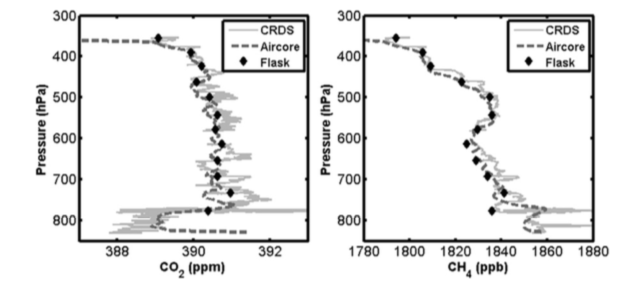
\includegraphics[width=1\linewidth]{7-data-analysis-and-results/img/ExpectedVerticalProfilesKarion.png}
    \end{align*}
    \caption{Pressure Profiles for (left) CO$_2$ and (right) CH$_4$ by Three Different Methods \cite{Karion}\label{fig:vertical-profile-karion}}
\end{figure}

The experiment's goal is to achieve the highest vertical resolution possible. Since the vertical resolution is determined by the length and the diameter of the tube \cite{Membrive}, a 300 m long tube will be used, consisting of 2 smaller tubes. One of 200 m length with \num{3e-3} m outside diameter and \num{1.3e-4} m wall thickness, and another one of 100 m length with \num{6e-3} m outside diameter and \num{1.3e-4} m wall thickness. For achieving higher stratospheric resolution, the tube with the smaller diameter will be used to sample the higher altitudes and the one with the bigger diameter for the lower ones.
Figure \ref{fig:resolution-lenght} by Olivier Membrive \cite{Membrive} compares the vertical resolution that can be expected with three different AirCores.

\begin{figure}[H]
    \begin{align*}
        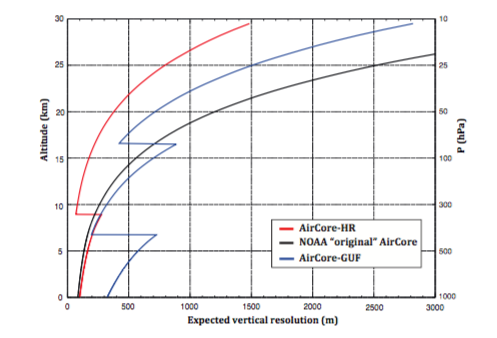
\includegraphics[width=1\linewidth]{7-data-analysis-and-results/img/ResolutionVslength.png}
    \end{align*}
    \caption{Comparison of the Vertical Resolutions That can be Expected with Different AirCores, After 3h Storage Time Before Analysis \cite{Membrive}\label{fig:resolution-lenght}}
\end{figure}

The High-Resolution AirCore-HR (red line),\cite{Membrive}, is a combination of two tubes. One of 200 m and one of 100 m.

The NOAA 'original' CAC, \cite{Karion}, (black line) is a 152 m long tube and the AirCore-GUF (designed and developed at Goethe University Frankfurt), (blue line) is a combination of three tubes, 100 m long in total.

The longer AirCore, AirCore-HR, achieved a higher resolution throughout the whole sampled air. 

In addition, the vertical resolution depends on the the mixing inside the tube. 

The experiment takes into account two types of mixing. Molecular diffusion and the shear flow diffusion, known as Taylor dispersion. The effect of molecular diffusion is described by the root-mean-square of the distance of molecular travel, 
\begin{equation}
    X_{rms} = \sqrt{2Dt}
\end{equation}
where, D is the molecular diffusivity of the molecule in the surrounding gas, and t is the time over which travel occurs, \cite{Karion}.
For the tubing dimension that will be used in this experiment, the flow of air through the CAC, will be laminar. In such a flow, a parabolic velocity profile exists inside the tube, causing longitudinal mixing (Taylor dispersion). 

Before the experiment is recovered, only molecular diffusion will affect the sample, but during analysis both molecular diffusion and Taylor dispersion will affect the sample. Combining both of them, an effective diffusion coefficient can be calculated as,
 \begin{equation}
     D{eff} = D + \frac{a^2\overline{V^2}}{48D}
 \end{equation}
where D is the molecular diffusivity, a is the tube's inner radius, and $\overline{V}$ is the average velocity \cite{Membrive}. The first term translates into the longitudinal direction, while the second one is the Taylor dispersion.

The exact flow rates are to be decided at a later stage of the experiment.

Finally, storage time, that is the time from the moment the tube is sealed until the end of the analysis, is a key factor that affects the experiment's results in terms of resolution.

Figure \ref{fig:resolution-time} shows the effect of time delay between landing and analysis, on the expected vertical resolution. 
\begin{figure}[H]
    \begin{align*}
        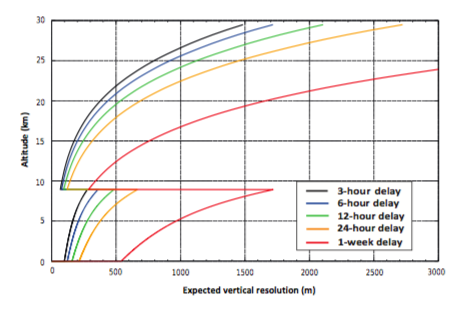
\includegraphics[width=1\linewidth]{7-data-analysis-and-results/img/ResolutionVsTime.png}
    \end{align*}
    \caption{Expected Vertical Resolution of AirCore-HR, for a Storage Time of 3h (black), 6h (blue), 12h (green), 24h (orange) and 1 week (red) \cite{Membrive}\label{fig:resolution-time}}
\end{figure}

It is clear that the sooner the samples are going to be analyzed, the better the results for the vertical resolution of the CAC sample. At an altitude of 20 km the resolution decreases significantly from 300 m to 500 m for 6h and 12h of delay, respectively, \cite{Membrive}. But even after a week of storage, a vertical profile can still be achieved with lower resolution.

Based on past BEXUS projects, the time to experiment recovery is estimated at 12 to 24 hours, if not multiple days. As such, it is expected that the desired vertical resolution of gas analysis will favour AAC configuration over that of CAC due to mixing of gases in the latter configuration, resulting in poorer vertical resolution.

The maximum vertical resolution for the AAC is capped at 500 m. This will be achieved assuring the airflow intake rate. For Ascent Phase, a nominal speed of 5 m/s is considered, which means that it will take 100 seconds to fill up a 3 L sampling bag while ascending 500 m, and therefore the airflow intake rate should be of approximately 1.8 L/min. For Descent Phase, the nominal speed is assumed to be 8 m/s. While descending 500 m a 3 L sampling bag will be filled in 62 seconds. However, considering the fact that the pump will not have the same efficiency at higher altitudes, the sampling time may be longer and the airflow intake rate may be higher. The exact numbers will be included in the upcoming version of the SED.  

For a 500 m of vertical displacement, the horizontal resolution of the AAC has been approximated based on past BEXUS flights data obtained from the BEXUS manual \cite{BexusManual}. The average horizontal resolution obtained for Ascent Phase is 588m and for Descent Phase is 186.5 m. This means that the square area covered by the sample will be 500 m x 588 m and 500 m x 186.5 m for ascent and Descent Phases respectively.

It is expected that the AAC will serve as model enabling a cost-effective large scale deployment scheme for regular high altitude greenhouse gas measurement. Unlike CAC, the design of AAC will not impose experimental restrictions based on the proximity of infrastructure for shipping and analysis. As such, a successful proof of concept of AAC sampling system will serve as a basis to enable reliable cost-effective measurements in remote areas.


